\documentclass[11pt,a4paper]{article}

\renewcommand{\figurename}{図}
\usepackage{mathtools}
\usepackage{setspace}
\onehalfspacing
\usepackage[top=1.75in, left=1.55in, bottom=1.75in, right=1.55in]{geometry}

\begin{document}

\noindent
非凸性と履歴効果\\
\ \\
\ \\
\ \\

経済モデルでは,多くの場合,消費者の選好や企業の生産技術について凸性が仮定される.
凸性の仮定は,
経済主体の行動を特徴付けることを容易にし,
競争市場のような分権的な資源配分メカニズムの有用性を担保するものである.
一方で,ある種の外部性が経済に存在する場合には凸性の仮定が満たされず,
標準的なモデルの分析手法がそのまま適用できないことが知られている(Starrett, 1972).
また,\underline{非凸性}は自然界に見られる正のフィードバック効果によっても生じるため,
近年では生態系の\underline{レジームシフト}の文脈で関心を集めている.

\noindent\textbf{●浅い湖とレジームシフト}\hspace{0.5em}
正のフィードバック効果が非凸性を生じさせるメカニズムは,
単純なモデルを用いて示すことができる.
時点$t$において
ある生態系に蓄積されている汚染物質のストックを$z(t)$,
外部からの汚染流入量を$x(t)$で表わす.
すると汚染物質の動学は,
$\dot{z}(t)$を時間あたりの変化量として,一般に
\begin{equation}\label{eq:z}%
  \dot{z}(t) = f(z(t)) + x(t)
\end{equation}
のようなモデルで表現できる.
関数$f$は汚染物質に対する自然の応答を捉えるもので,
その形状はシステムによって異なる.
例えば\underline{浅い湖}を考えた場合,
水質汚染物質(リン)の動学は,おおむね
\begin{equation}\label{eq:f}%
  f(z) := -\delta z + \alpha\frac{z^{2}}{1+z^{2}}
\end{equation}
のような$f$によって表現できるとされる(Scheffer, 1997).
%ただし,$\delta >0$かつ$\alpha \geq 0$とする.
\eqref{eq:f}の第1項は
湖外への流出や湖底への堆積を通じた自然浄化能力を表現しており,
負のフィードバック($z$について減少関数)である.
一方,第2項は正のフィードバック($z$について増加関数)で,
主に湖底に堆積したリンが再び水中に溶け出す現象を捉えている.
パラメタの$\delta >0$と$\alpha >0$は,
それぞれ負のフィードバックと正のフィードバックの強度を表わす.

話を簡単にするために
外部からの流入量は一定である($x(t)=x\geq 0$)とすると,
定常状態(長期的な均衡)における汚染ストックの量は$f(z)+x = 0$,つまり
\begin{equation}\label{eq:ss}%
  -\delta z + \alpha\frac{z^{2}}{1+z^{2}} + x = 0
\end{equation}
を満たす$z$によって特徴付けられる.
定常状態における$z$が環境負荷$x$に対してどのように反応するかを考えると,
まず正のフィードバックの相対的な強度が十分に弱い($\alpha/\delta\approx 0$)時には,
\eqref{eq:ss}の第2項はほとんど無視できるから,
$z$は$x$に線形的に反応することが分かる.
一方で,
正のフィードバックがある程度の強度を持つ($\alpha/\delta\approx (4/3)^{3/2}$)場合,
\figurename~\ref{fig:nonconvex_lake}の左側のパネルにあるように, 
定常状態における$z$と$x$の関係は強い非線形性を示すようになる.
このようなケースでは,環境負荷のレベルがある閾値(図中の$\bar{x}$)を超えると,
システムの状態に急激な変化(レジームシフト)をもたらす.
%
\begin{figure}[t]\centering%
  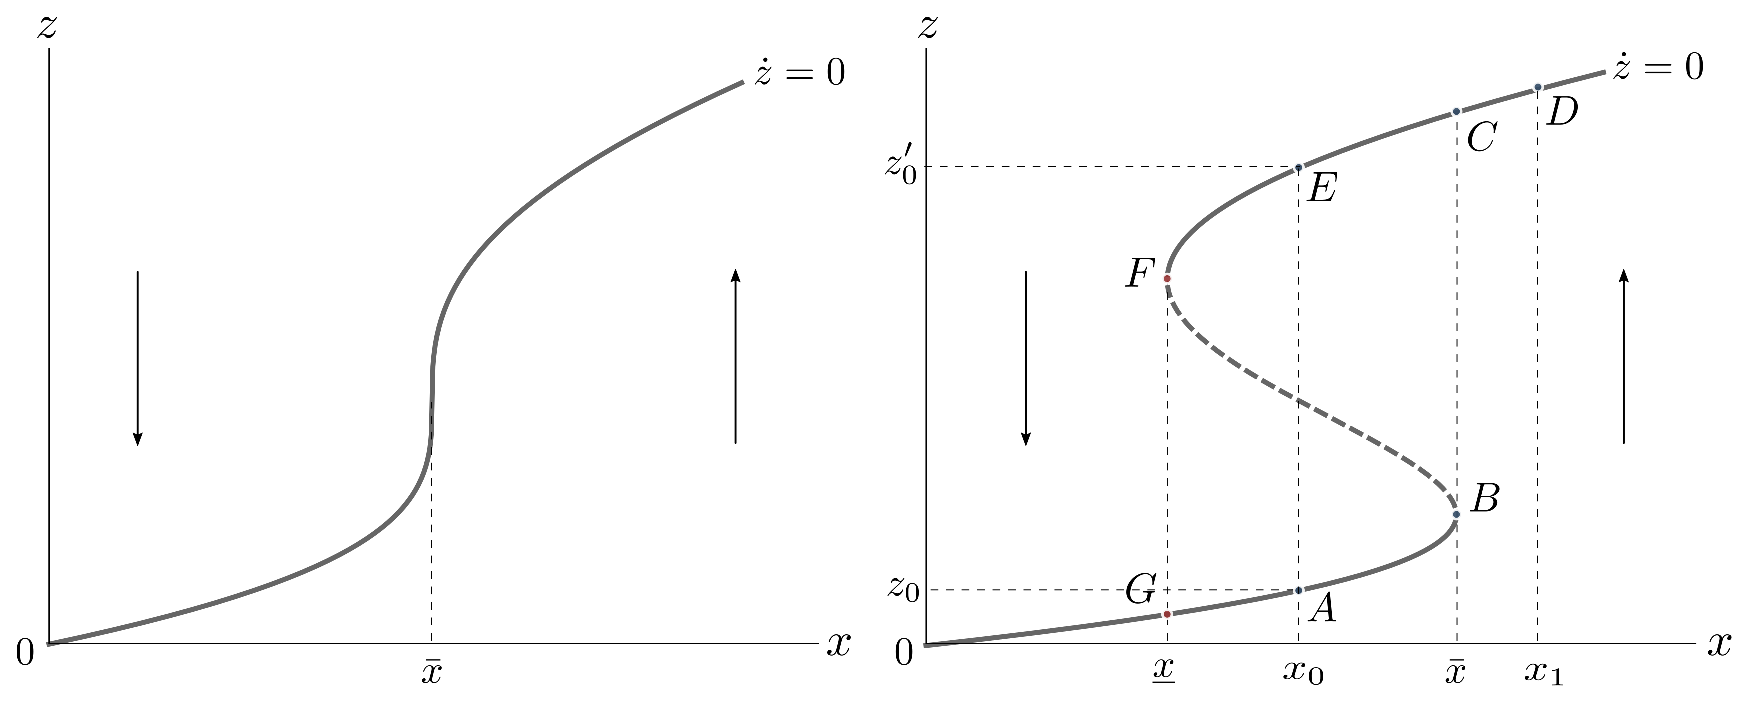
\includegraphics[width=380pt]{figures/fig_nonconvex_lake_b.eps}
\caption{レジームシフトと履歴効果}
\label{fig:nonconvex_lake}
\end{figure}

\noindent\textbf{●履歴効果と不可逆性}\hspace{0.5em}
さらに,正のフィードバックが十分に強い($2>\alpha/\delta> (4/3)^{3/2}$)場合には, 
$z$と$x$の関係は\figurename~\ref{fig:nonconvex_lake}の右側のパネルのようになり,
\underline{履歴効果}と呼ばれる現象が生じる.
履歴効果とは,いったん環境負荷を強め過ぎてしまうと,
負荷のレベルを当初の水準に戻してもシステムの状態が元に戻らないことを言う.
例えば,$x_{0}$という環境負荷の下で汚染状態が$z_{0}$で安定している状況(図中の$A$)を考える.
この時,環境負荷を$x_{1}$まで強めると,
$\bar{x}$を超えた時点でシステムの均衡が$B$から$C$に移動し(レジームシフト),
長期的には$D$で安定する.
逆にその状態から環境負荷を弱めると,
$\bar{x}$を下回ってもシステムが安定的であり続けるため,
$x_{0}$まで負荷を弱めたとしても($A$ではなく)$E$に留まることになる.
システムを元の状態に戻すためには,
環境負荷をさらに低い水準(図中の$\underline{x}<x_{0}$)まで弱め,
$F$から$G$へと状態を移動させなければならない.

このモデルを用いると,システムに不可逆的な変化が生じる可能性を指摘することもできる.
例えば,正のフィードバックが極めて強い($\alpha/\delta > 2$)場合には,
(元に戻る方向の)レジームシフトの閾値$\underline{x}$が負の値となる.
そのようなケースでは,
いったんシステムが高水準の汚染状態で安定してしまうと,
外部からの環境負荷を完全に取り除いても原状を回復することは不可能である.
(阪本浩章)

\clearpage

\subsubsection*{引用参照文献}

\begin{enumerate}
  \item Scheffer, M. (2004) \emph{Ecology of Shallow Lakes}, Springer.
  \item Starrett, D. (1971) ``Fundamental nonconvexities in the theory of externalities,''
    \textit{Journal of Economic Theory}, 4(1), 180--199.
\end{enumerate}

\subsubsection*{索引語}

\begin{itemize}
  \item 非凸性(non-convexity)
  \item レジームシフト(regime shift)
  \item 浅い湖(shallow lake)
  \item 履歴効果(hysteresis)
\end{itemize}

\end{document}